\ifx\wholebook\relax \else

\documentclass[b5paper]{ctexart}
\usepackage[nomarginpar
  %, margin=.5in
]{geometry}

\addtolength{\oddsidemargin}{-0.05in}
\addtolength{\evensidemargin}{-0.05in}
\addtolength{\textwidth}{0.1in}

\usepackage[cn]{../prelude}

\setcounter{page}{1}

\begin{document}

\title{无理数}

\author{刘新宇
\thanks{{\bfseries 刘新宇} \newline
  Email: liuxinyu99@hotmail.com \newline}
  }

\maketitle
\fi

\markboth{无理数}{数的旅程}

\ifx\wholebook\relax
\chapter{无理数}
\fi

\epigraph{数学是上帝用来书写宇宙的文字}{伽利略}

公元前270年的夏至中午,这一天是一年中日照最长的一日,大约是现代历法的6月21日附近。埃及亚历山大港图书馆馆长埃拉托斯特尼正和一位来自赛印城\footnote{赛印(Syene)位于今天埃及南部的阿斯旺}的商人交谈。“我的老家是世上最干最热的地方。”商人说道:“我们打了很深的井汲水,每年的这个时候,阳光能射到井底呢。”听到这句话时埃拉托斯特尼却注意到了到广场上纪念碑的影子。为什么会这样呢?除非大地不是平坦的,而是球形。他询问哪个商人:“从赛印城到亚历山大有多远的路程?”“有5000斯塔蒂亚\footnote{斯塔蒂亚(Stadia)是古希腊的长度单位,约和158米}。”埃拉托色特尼测量了立在地上的杆子和影子的长度,发现杆子的长度是影子长度的8倍。他于是按照\cref{fig:eratosthenes-earth}进行了计算。

\begin{figure}[htbp]
 \centering
 \subcaptionbox{太阳在夏至直射北回归线上的赛印城\label{fig:eratosthenes-earth}}{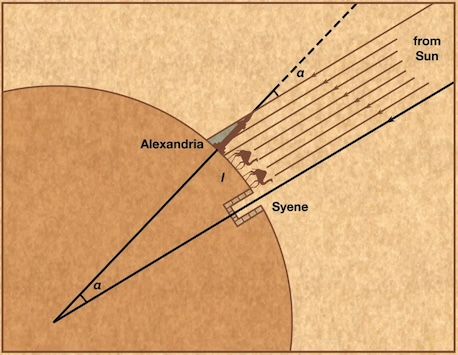
\includegraphics[scale=0.35]{img/eratosthenes-earth}}
 \subcaptionbox{太阳照射亚历山大的角度为$\alpha$\label{fig:atan8}}{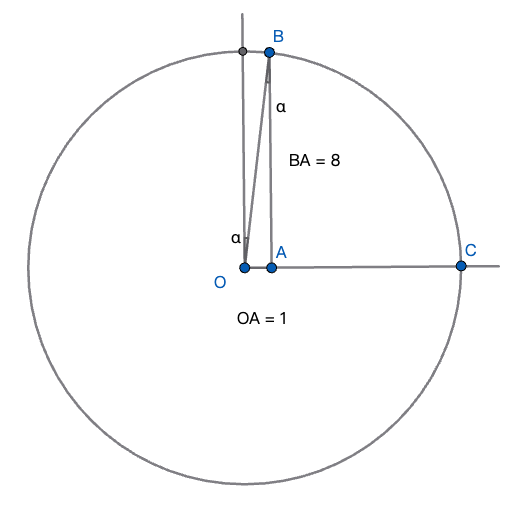
\includegraphics[scale=0.32]{img/atan8}}
\end{figure}


\section{万物皆数}
音乐与数似乎毫无关联,但毕达哥拉斯却发现了它们背后竟有奇妙的规律。他从中得到启发并大胆推测“万物皆数\footnote{英文All is number}”——世间万物都可以用数或数的比例来理解。

All is number.

\section{勾股定理}
Pythagoras theorem and varies of proofs.

\section{数论}
Euclid's proof to the Pythagoras triples.
Euclid and Elements
Perfect numbers and Even perfect numbers theorem (Euclid), Fermat numbers and Mersenne primes.

\section{无理数}
Discovery of irrational number, square root of 2 and n.
Compass and ruler construction I
Golden ration and Fibonacci series.

\section{欧几里得算法}
Euclidean algorithm,
It's extension and Bezout identity.
Geometric meaning of Euclidean algorithm.
Continue fraction and Euclidean algorithm.
Uncommensurable and irrational numbers, (Elements)

\section{更多的无理数}
Compass and ruler construction II,

polygon construction (pentagon, 17-gon)

Solving polygon construction with number theory, Fermat numbers, Perfect numbers, and Wantzel theorem.

\section{圆周率}
pi as an irrational number

\section{思想之剑}
Dedekind cut

\ifx\wholebook\relax \else
\section{参考答案}
\shipoutAnswer

\begin{thebibliography}{99}
\subimport{inc/}{bib-zh-cn}
\end{thebibliography}

\expandafter\enddocument
\fi
